\documentclass[11pt,a4paper]{article}

\usepackage{url,,}
\usepackage{graphicx}
\usepackage{hyperref}
\usepackage{amsfonts}
\usepackage{amssymb}
\usepackage{amsmath}
\usepackage{multirow}
\usepackage{listings}
\usepackage{fullpage}
\usepackage{fancyhdr,a4wide}
\usepackage{makeidx}
\usepackage{placeins}
%\usepackage[procnames,noindent]{lgrind}

\lstset{ %
language=VHDL,                % choose the language of the code
basicstyle=\footnotesize,       % the size of the fonts that are used for the code
showstringspaces=false,         % underline spaces within strings
%numbers=left,                   % where to put the line-numbers
%numberstyle=\footnotesize,      % the size of the fonts that are used for the line-numbers
%stepnumber=1,                   % the step between two line-numbers. If it's 1 each line will be numbered
%numbersep=5pt,                  % how far the line-numbers are from the code
%backgroundcolor=\color{white},  % choose the background color. You must add \usepackage{color}
showspaces=false,               % show spaces within strings adding particular underscores
showtabs=false,                 % show tabs within strings adding particular underscores
escapeinside={\%*}{*)}          % if you want to add a comment within your code
}

\begin{document}	

\begin{titlepage}

\thispagestyle{fancy}
\lhead{}
\chead{
\large{\textit{
Informatics and Mathematical Modelling\\
Technical University of Denmark}}}
\rhead{}
\rule{0pt}{50pt}
\vspace{3cm}

\begin{center}
 	\huge{\textbf{02207 : Advanced Digital Design Techniques}}\\
 	\vspace{1cm}
 	\huge{Low-pass Filter (2 x 1-D)}\\
 	\vspace{1cm}
 	\huge{\textit{Examination Project}}\\
 	\vspace{1cm}
 	\huge{Group \textit{dt07}}\\
\end{center}

\vspace{4cm}

\begin{flushright}
	\LARGE{Markku Eerola (s053739)}\\
	\vspace{0.3cm}
	\LARGE{Rajesh Bachani (s061332)}\\
	\vspace{0.3cm}
	\LARGE{Josep Renard (s071158)}\\
\end{flushright}
\cfoot{\today}
\end{titlepage}

\newpage 
\tableofcontents

\newpage

\section{About the Report}
In this project, we have designed and implemented the architecture for an image filtering processor which uses a 3x3 filter to perform a convolution on the image of size 256x256 pixels.

Following is the work done by the authors.
\paragraph{Authors by Section}
\begin{itemize}
\item \textit{Rajesh Bachani} 
\item \textit{Josep Renard} 
\item \textit{Markku Eerola} 
\end{itemize}


The rest of the report is organized as follows. In section \ref{sec:design}, we explain the internal architecture of the processor. Then in section \ref{sec:sequencing}, we give the sequencing of the operations involved in the computation. This section explains the operations performed for memory initialization and the order in which the input memory is read and the output memory is read and written. Also, we here explain the order in which the memory is accessed, which are different for the horizontal and vertical movements of the filter mask. Section \ref{sec:controller} explains the design of the controllers at the input and the output. In section \ref{sec:synthesis}, we provide the results from the synthesis of the design in Design Vision. The section \ref{sec:results} contains the images obtained after convolution, and also a summary of the results from the synthesis. Finally, we end the report with section \ref{sec:limitations} with a short explanation on what we think are the limitations of the work done here, and how it could be extended.

\section{Design Architecture}
\label{sec:design}
%give the block design here. we need the following figure:
%a complete diagram of the processor - indicating the input and output signals, and also containing the internal blocks like the cache register,filter register, fsm_in, the multipliers, adders, mux, and fsm_out.
The overall design of the filter unit can be seen in figure \ref{fig:proc}. More detailed architecture can be seen in figure \ref{fig:procdetail}.

\begin{figure}[h]
	\centering
		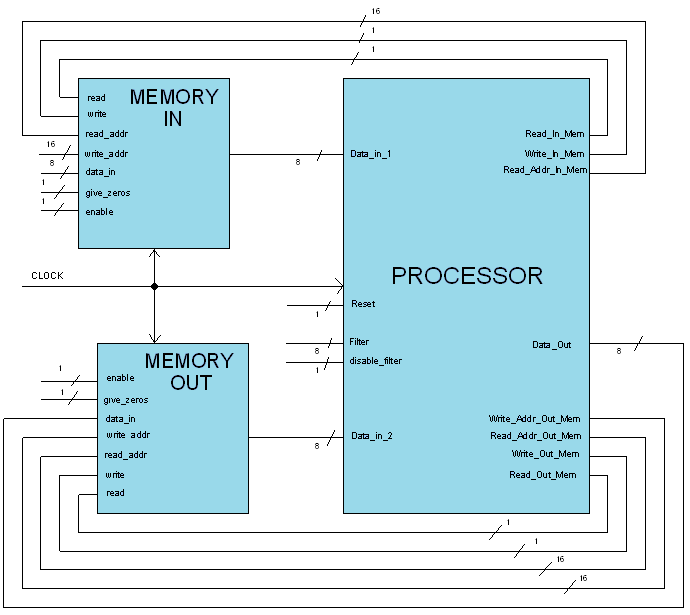
\includegraphics[width=4in]{./images/processador.PNG}
	\caption{Filter unit design}	\label{fig:proc}
\end{figure}

\begin{figure}[h]
	\centering
		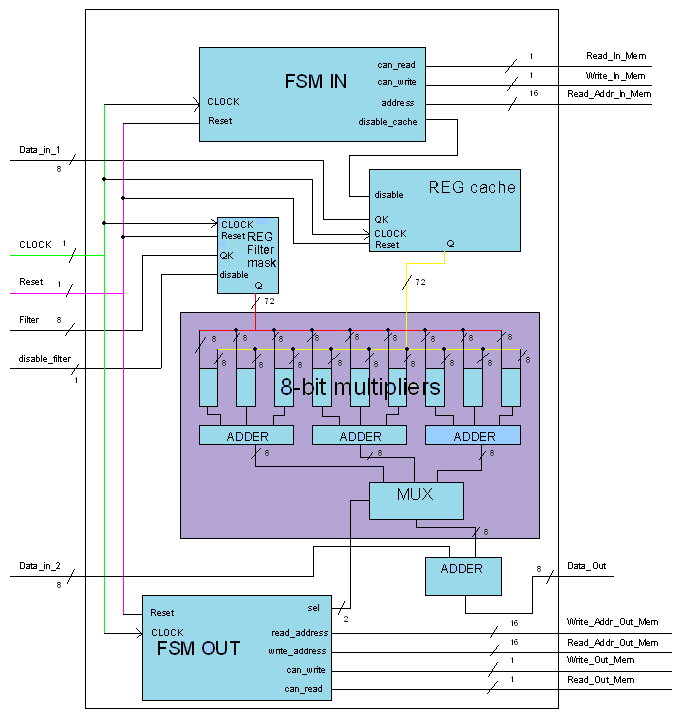
\includegraphics[width=4in]{./images/insideproc.PNG}
	\caption{Processor architecture}	\label{fig:procdetail}
\end{figure}

%here we should mention the details about the data path, bit widths etc. 
%we should give a brief explanation of each of the components in the architecture - just a couple of lines explanation should be good enough. 
%also we should explain the purpose of each of the input and output signals of the memory and the processor.

\FloatBarrier
\section{Sequencing of Operations}
\label{sec:sequencing}

This section contains a description of the sequence in which the processor performs the operations needed for convolution of the image. 

\subsection{Memory Initialization}
%how the initialization is done - the input FSM keeps the write of the input memory till 65526 clock cycles - so all the pixels are read from the hex file.
%in the meantime, the output FSM keeps the write signal of the output memory to 1 and it is initialized with 0.

%In our case we have an image on format .hex, is the values of the image on hexadecimal, 2 values of 4 bits, 8 bits total, and we have to pass all the image to the memory so there are 65536 values on our image, so the processor are going to spend this amount on clock cycles, but we need too another memory to store the new values of the convolution for the next vertical filter pass. For this task we have a final state machine that is in charge to create an address and store the value on the memory with this address. So now we have to create two memories, the first one that we call memory in are going to be the values of the image to filter with their correspondent address, the final state machine generate the address and give to the memory the value of the image with their correspondent address, at the same time because are different state machine and memory, the space for the filtered image is created in a parallel way, but now the difference between the first one is that we want the memory empty, all with zeros, and we use the processor to make this operation, the final state machine for the output create the addresses and has the property to say the multiplexor of the final output which one wants, and one of the outputs is all zeros, so with that the processor knows that in this time period for initializing the memory out throws by Data\_out a value 0 all the time.
%When the 65536 clock cycles are ended the memory in is with the values of the image and the memory out empty, all with values zeros.	

\subsection{Memory Read and Write by Processor}
\label{sec:memreadwrite}
%Once the initialization is done, 
% 1. the input fsm reads 3 pixels - and then waits for 9 clock cycles
% 2. the output fsm starts when the input fsm becomes idle - and runs the sequence read-idle-write 3 times.
%give picture from modelsim here showing how the two fsms synchronize.

There are two controllers as part of the processor, the Input Controller and the Output Controller (indicated by FSM\_In and FSM\_Out in figure \ref{fig:procdetail}). The Input Controller is responsible for reading pixels from the input memory, which holds the original image. On the other hand, the output controller is responsible for reading as well as writing the computed pixels from and to the output memory. The output memory holds the pixels of the convoluted image. 

It is very important that these two controllers be well synchronized with each other, so the operations are performed smoothly, and there is no data loss. In particular, when the Input Controller is active, the Output Controller should not perform any operation. This is because until the Input Controller has read the next 3 pixels (for the 3x3 filter; it would be $n$ for nxn filter) from the input memory, the convolution is not stable, and so the Output Controller cannot write anything to the output memory. The vice-versa case is also true. So, when the Output Controller is active, the Input Controller should be inactive. This is because while the output memory is being written by the Output Controller, if the Input Controller reads new pixels, then the already computed values would be overwritten, and the synchronization is disturbed completely.

Hence we have chosen the approach in which at no point of time, would both the Controllers be active. This can be seen from the figure \ref{fig:controllerreadwrite.jpg}.


% AN image here. Name it controllerreadwrite.jpg

\subsection{Memory Access Sequence}
\label{sec:memoryaccess}
%mention the sequence of the memory access from the input fsm and the output fsm
\begin{figure}[h]
	\centering
		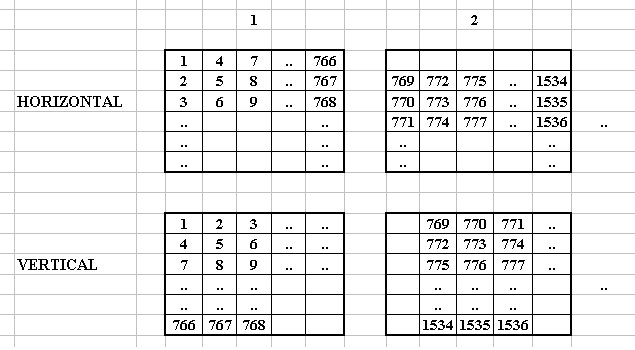
\includegraphics[width=5in]{./images/memoryAccess.PNG}
	\caption{Sequence of Memory Address Access}	
	\label{fig:memaccess}
\end{figure}


%For the memory sequence we use a particular way, we want to access to the memory the less time possible, so we have created one kind of memory cache inside the processor, the cache consist in one ShiftRegister for store 9 pixels, the number of pixels that we need to filter with our mask of 3x3, and on the beginning the final state machine take from the memory 9 values, for fill all the cache, but on the next clock cycle only take 3 values from the memory, the next column if we are on the horizontal pass (Figure 1(file horizontal pass)) or the next row if we are on the vertical pass (Figure 2(file vertical pass)) as we can see. But the sequence has a particular thing, when the values of the memory arrives to the end of the picture now doesn't work the shiftregister because we have to come back to the beginning and start again, so when the image values seized from the memory, last column on the horizontal pass and last row on the vertical pass, there are another time 9 lectures from the memory to fill up all the shift register and continue the same mechanism like l say before.
%

\section{Finite State Machines}
\label{sec:controller}

The following subsections explain the finite state machines describing the Input and the Output Controllers.

\subsection{Input Controller}

The Input Controller has the following 16 states.
\begin{enumerate}
\item State \textit{init}. This is the initialization state of the controller. The next state is \textit{init\_in\_memory\_1}.

\item State \textit{init\_in\_memory\_1}. This state performs the initialization of the input memory. The Controller puts the  \textit{can\_write} signal to \textit{1}, so that the byte read from the $.hex$ file is written to the \textit{Data\_In} of the input memory. The address to which the byte should be written is also given by the Controller, through the signal \textit{address}. The next state is \textit{init\_in\_memory\_2}.

\item State \textit{init\_in\_memory\_2}. This state does the same thing as the previous state, and it increments a counter. Once the value of the counter is greater than 65536, which means that the entire memory has been written, the state changes to \textit{h\_read\_1}.

\item State \textit{h\_read\_1}. This state performs the read operation from the input memory for one pixel. The signal \textit{can\_write} is set to \textit{1}. The next state is \textit{h\_read\_2}.

\item State \textit{h\_read\_2}. This state performs the read operation from the input memory for one pixel. The next state is \textit{h\_read\_3}. The signal \textit{disable\_cache} is set to \textit{0} here, since from now we want the cache to start loading the values from the input memory. 

\item State \textit{h\_read\_3}. This state performs the read operation from the input memory for one pixel. The next state is \textit{h\_cache}.

\item State \textit{h\_cache}. This state is used as a delay. The signal \textit{disable\_cache} should be delayed by one clock cycle as compared to the signal \textit{can\_read} since the byte from the memory comes one clock cycle after the \textit{can\_read} is active. The signal \textit{can\_read} is set to \textit{0} here. The next state is \textit{h\_wait}.

\item State \textit{h\_wait}. This state is used as a wait state, during which the Output FSM is active. Also, the \textit{disable\_cache} signal is set to \textit{1} here, so that no more values from the memory are read into the cache, until the Input Controller gets active again. The next state is \textit{h\_temp}.

\item State \textit{h\_temp}. This state is also the wait state, and the finite state machine keeps shuttling between this state and the previous state, for 27 clock cycles. Once the Output Controller writes the new pixels to the output memory, the wait time is over, and the next state is set to \textit{v\_read\_1} and the vertical reading for the memory is started.

The states for vertical movement are kept separate from the states for the horizontal movement. This is because the order in which the addresses are generated for the \textit{address} signal, are different in both the movements (as also shown in figure \ref{fig:memaccess}). The purpose of the following states is the same though, with only the address values being different, so we skip the explanation.
\item State \textit{v\_read\_1}. 

\item State \textit{v\_read\_2}. 

\item State \textit{v\_read\_3}. 

\item State \textit{v\_cache}. 

\item State \textit{v\_wait}. 

\item State \textit{v\_temp}.

\item State \textit{exit\_in}. This is the exit state of the finite state machine.

\end{enumerate}


\subsection{Output Controller}
The Output Controller has the following 18 states.
\begin{enumerate}
\item State \textit{init}. This is the initialization state of the controller. The next state is \textit{init\_out\_memory\_1}.

\item State \textit{init\_out\_memory\_1}. This state initializes the output memory to \textit{0}. The controller puts the \textit{can\_write} signal to \textit{1} and the \textit{write\_address} is incremented every time in the state. The next state is \textit{init\_out\_memory\_2}.

Important to note here, that the output memory is initialized by zeros, since the \textit{Data\_In\_2} signal coming from the output memory is set to zero, using the \textit{give\_zeros} signal of the output memory. Also the multiplexer in this state gives zero since the select is forced to `11' by the controller. Hence the \textit{Data\_Out} of the processor is always zero in this state.

\item State \textit{init\_out\_memory\_2}. This state performs the same function as the previous state. A counter is maintained which if greater than 65536 indicates that the memory is initialized. Then the next state is \textit{h\_init\_1}

\item State \textit{h\_init\_1}. This state is created in order to wait for the cache shift register to get the pixels from the input memory. Actually, when the Input Controller finishes reading a line in the memory, during any of the horizontal or vertical movements, the Output Controller must wait for the time till the cache is filled with the new 9 pixels. The next state is \textit{h\_init\_2}.

\item State \textit{h\_init\_2}. This state performs the same function, and waits till the 9 pixels are filled in the cache shift register. This takes 27 clock cycles, since the Input Controller also remains idle in between. Once this is done, the next state is set to \textit{h\_read\_1}. 

\item State \textit{h\_read\_1}. This state puts the \textit{can\_read} signal to \textit{1}. Also, the corresponding \textit{read\_address} is set. The next state is \textit{h\_read\_write}.

\item State \textit{h\_read\_write}. In this state, the Controller remains idle, so that data is recieved from the output memory in the next clock cycle. The next state is \textit{h\_write\_1}. 

\item State \textit{h\_write\_1}. This state forces the adder to be selected, by changing the \txtit{sel} signal. The old pixel from the output memory and the new pixel from the adder are added. The signal \textit{can\_write} is set to \textit{1} and the \textit{write\_address} is set to the same value as the \textit{read\_address} in the previous state. If the end of the row or column is reached in the memory, the next state is \textit{h\_init\_1}. Else the next state is \textit{h\_wait\_1}. Also, if the end of the image is identified, then the vertical movement begins, and in that case the next state is set to \textit{v\_init\_1}

\item State \textit{h\_wait\_1}. In this state, the Controller waits for the Input Controller to read 3 new pixels from the input memory. The next state is \textit{h\_wait\_2}.

\item State \textit{h\_wait\_2}. This state performs the same function as the previous state. If 3 clock cycles are over, i.e. if the Input Controller has read 3 new pixels, then the Controller gets active again, and the next state is set to \textit{h\_read\_1}.

Again, we avoid giving explanation for the states during the vertical movement, since they all perform the same function as the states occuring during the horizontal movement.
\item State \textit{v\_init\_1}. 

\item State \textit{v\_init\_2}. 

\item State \textit{v\_read\_1}. 

\item State \textit{v\_read\_write}. 

\item State \textit{v\_write\_1}. 

\item State \textit{v\_wait\_1}. 

\item State \textit{v\_wait\_2}.

\item State \textit{exit\_in}. This is the exit state of the finite state machine.

\end{enumerate}


\FloatBarrier
\section{Synthesis}
\label{sec:synthesis}
%present the results from the various reports here. 
% the critical path
% area 
% power dissipation
We synthesized the design using four different clock periods, namely 7ns, 5ns, 3ns and 2ns, and let Design Vision try to optimize the design for speed to get the fastest possible design. Turns out 2ns is the minimum clock period for our design, Design Vision was not able to synthesize a faster design even when we tried. To get meaningful power reports we simulated switching activity with the VSS Simulator and the activity was passed on to Design Vision. On top of power reports we also obtained area and timing reports from the design on all four clock cycles. The actual reports can be seen in the appendix, but a summary of the results can be seen in table \ref{tab:synth}.

\begin{table}[h]
	\caption{Summary of Design Vision reports}
	\begin{center}
		\begin{tabular}{|l|l|l|l|l|l|l|} \hline
			\textbf{T}_{C} [ns]	& \textbf{P}_{stat}	[mW] & \textbf{P}_{dyn} [mW]	& \textbf{P}_{tot} [mW] & \textbf{A}_{comb} [\mu m^2]& \textbf{A}_{tot} [\mu m^2] & \textbf{T}_{cp} [ns] \\ \hline
			7 & 0.11 & 1.60 & 1.71 & 44067 & 53079 & 4.7 \\ \hline
			5 & 0.11 & 1.71 & 1.82 & 44067 & 53079 & 4.7 \\ \hline
			3 & 0.13 & 2.19 & 2.32 & 49595 & 58611 & 2.9 \\ \hline
			2 & 0.20 & 2.60 & 2.80 & 58668 & 67700 & 1.9 \\ \hline
			
		\end{tabular}
	\end{center}
	\label{tab:synth}
\end{table}

\FloatBarrier
\section{Results}
\label{sec:results}

%put the convoluted and the original image here to show the results.

\begin{table}[h]
	\caption{Summary}
	\begin{center}
		\begin{tabular}{|p{1cm}|p{2cm}|p{2cm}|l|l|} \hline
			\textbf{T}_C [ns] & \textbf{Critical Path} [ns] & \textbf{N. cycles} (256 x 256) & \textbf{E}_{pc} [mW/MHz] & \textbf{AREA} [\mu m^2] \\ \hline
			7 & 4.7 & 3121152 & 0.01197 & 53079 \\ \hline
			5 & 4.7 & 3121152 & 0.00910 & 53079 \\ \hline
			3 & 2.9 & 3121152 & 0.00696 & 58611 \\ \hline
			2 & 1.9 & 3121152 & 0.00560 & 67700 \\ \hline
		
		\end{tabular}
	\end{center}
	\label{tab:conclusion}
\end{table}


\section{Limitations and Extensions}
\label{sec:limitations}

We have designed and implemented the architecture for an image filtering processor which uses a 3x3 filter to perform a convolution on the image of size 256x256 pixels. Though the results of the convoluted image look promising, as shown in section \ref{sec:results}, we are aware of some of the limitations of the work. Given more time, we would have liked to add the following missing aspects into the project.

\begin{enumerate}
\item We have just been able to implement the 3x3 filter for the convolution. Though, it was proposed that we would implement the higher dimension filters as well, including 5x5, 7x7 and 9x9, we were not able to do so, due to the initial problems we faced in the implementation of the 3x3 filter itself. We believe the results obtained in the section \ref{sec:results}, in the form of the convoluted image could be better if the dimension of the filter is higher. In those cases, the blur effect on the image would be clearly evident, as compared to the case of the 3x3 filter. We would like to briefly mention how the design of the processor would be modified if we wish to convolute the image using higher dimension filters. If we consider the dimension of the filter as nxn, then we have the following:
	\begin{itemize}
		\item Number of Adders = $n^2$
		\item Number of Multipliers = $n$
		\item Size of the Cache Shift Register = $n^2$
		\item Multiplexer would have $n$ inputs and $1$ output.
		\item Select signal from the Output Controller would be 3 bits for 5x5 and 7x7, and 4 bits for 9x9 filter.
	\end{itemize}	
	
	In addition the synchronization of the Input and the Output Controllers would change due to the number of clock cycles required to get $n$ new pixels from the memory and compute the output for n pixels at a time. This means the cases described in section \ref{sec:memreadwrite} would now be the following:
	
	
\item It is assumed that the filter is symmetric along the two dimensional x and y axes. We need this since the indices of the filter which need to be multiplied with the image pixels would change in horizontal and vertical movements. For simplicity therefore, we have made this assumption.
The solution to this problem is quite simple though. We just need to have separate caches in the processor which hold the filter values in a different order. For horizontal movement we would use one cache, while the other one would be used for the vertical movement.

\item The mechanism which we have designed for the accessing the memory is ofcourse not the best way. Since we began the implementation with the sequence explained in the section \ref{sec:memoryaccess}, we did not change it later. Though, we realized that this is not an efficient way, since it consumes a high number of clock cycles in order to run through the entire image of 256x256 pixels.
\end{enumerate}	

\end{document}